% Provenance (never printed): see sources/outline_sources.md (Year 3:
% energy-balance models, the one-layer model recalled; ice-albedo feedback
% and multiple equilibria; how general circulation models are built and
% evaluated).
% Brief: sources/book5/BRIEFS.md, ch. 22. Curves from
% figdata/bachelor-3/budyko_sellers.py (the zero-dimensional model and
% Budyko's latitudinal model; the brief's ebm_0d is folded into it) and
% two_layer.py. Exercise and problem values in the Book 5 scratch calculator
% calc/ch22.py. The model planet, model X and the ensemble of exercise 12 are
% invented.
\chapter{气候模式}\label{ch:b3:climate-models}

取到达地球的太阳辐射，全球平均为 \qty{340}{W/m^2}，
以及一条地球向太空发出红外辐射的规律，该规律
拟合自三十年观测的再分析资料。令行星反照率由
开阔陆地与海洋的反照率，随地表降温升至冰的反照率。令两种
通量相等，由此方程有三个解：一颗行星温度为
\qty{14}{\celsius}，接近真实地球的平均值；另一颗行星温度为
\qty{8}{\celsius}；再一颗温度为 \qty{-46}{\celsius}，整个星球从极
到极冰封。气候模式，从寥寥数行的方程
到运行于最大型计算机上的程序，都是用来探讨某颗行星具有何种气候、它如何
形成这种气候，以及能量收支受扰动时它如何变化。
% ledger: nasa:solar-mean, data:b5-ncep-air, data:b3-ncep, budyko69:albedo

\begin{recall}
黑体、斯特藩–玻尔兹曼定律、温室效应以及
大气单层模式见于物理学教材；反照率与
地球能量收支见于中学教材。向外长波
辐射、发射温度与经向热量输送见于
本科一年级分册，见其关于辐射与热量输送的章节。
冰–反照率反馈与雪球地球见于本科二年级分册，
见其关于前寒武纪地球的章节；有效辐射强迫、
气候反馈参数 $\lambda < 0$、平衡气候
敏感度（ECS）与瞬态气候响应（TCR）见于
其关于人为气候变化的章节；数值天气预报与
集合预报见于其关于天气系统的章节。旋转地球上的运动
方程，连同\omterm{def:b3:gfd-foundations:hydrostatic}{静力近似}，见于
第~\ref{ch:b3:gfd-foundations}~章。
\end{recall}

\section{行星的能量收支}\label{sec:b3:climate-models:zero-d}

对整个球面并取一年平均，大气顶部每平方米
接收的太阳辐射为 $Q = S_0/4 = \qty{340}{W/m^2}$，即太阳辐照度的
四分之一，$S_0 = \qty{1360}{W/m^2}$。比例为 $\alpha$ 的部分，即
行星反照率，被反射；其余 $Q(1 - \alpha)$ 被吸收，
须以红外辐射形式返回太空。黑体的发射量为 $\sigma
T^4$；地球的向外长波辐射（OLR）较小，原因是
温室效应；在地球上所见的地表温度范围内，
它近似为一条直线，
\[
\text{OLR} = A + BT ,
\]
式中 $T$ 为以摄氏度计的地表温度。1969 年，布迪科拟合出
这一规律，所用为 260 个台站算得的向外辐射，并修正了
云量 $n$：$I = a + bT - (a_1 + b_1T)n$，$a = 14.0$，$b = 0.14$，$a_1 =
3.0$ 与 $b_1 = 0.10$，单位为 \unit{kcal.cm^{-2}}（每月），散布小于
\qty{5}{\percent}。取平均云量为 0.5 时，给出 $A =
\qty{199}{W/m^2}$ 与 $B = \qty{1.43}{W.m^{-2}.\celsius^{-1}}$。
取 NCEP--NCAR Reanalysis~1 在 1991--2020 年的年平均\omterm{def:b3:atmospheric-dynamics:eddy}{纬向平均}，按面积加权，
得 $A = \qty{211.9}{W/m^2}$ 与 $B = \qty{1.816}{W.m^{-2}.\celsius^{-1}}$，
围绕该直线的散布为 \qty{10}{W/m^2}。这些数值
在下文中均被采用。
% ledger: nasa:solar-mean, budyko69:olr, data:b5-ncep-air, data:b3-ncep

\begin{definition}[能量平衡模型]\label{def:b3:climate-models:ebm}
称\emph{能量平衡模型}\index{能量平衡模型}为一种气候模式，
它计算地表温度——可以是全球单一的平均值，或
各纬度上的平均值——取决于被吸收的太阳辐射、
射向太空的红外辐射，以及（若温度随纬度而变）
被输送至两极的热量之间的平衡。其零维形式为
\[
C\,\frac{\mathrm dT}{\mathrm dt} = Q\big(1 - \alpha(T)\big) - (A + BT) ,
\]
式中 $C$ 为随地表一同升温的那部分系统的单位面积
热容。
\end{definition}

取 $\alpha = 0.30$，平衡温度为 $T = (238 - 211.9)/1.816 =
\qty{14.4}{\celsius}$；再分析资料的面积平均为
\qty{14.2}{\celsius}。一个强迫 $F$，例如
二氧化碳含量变化所产生的强迫，加在方程右端。平衡点附近的响应
由本科二年级分册中的气候反馈参数 $\lambda$ 决定：
在反照率固定的情形下，$\lambda = -B$。
% ledger: earth:albedo, data:b5-ncep-air

\begin{theorem}[单箱气候的响应时间]\label{thm:b3:climate-models:response}
设气候处于平衡态，且恒定强迫 $F$ 在
$t = 0$ 时接入。若偏离平衡态的量 $T'$ 满足 $C\,\mathrm
dT'/\mathrm dt = F + \lambda T'$，其中 $C > 0$ 且 $\lambda < 0$ 为常数，
则
\[
T'(t) = -\frac{F}{\lambda}\Big(1 - \mathrm e^{-t/\tau}\Big), \qquad
\tau = -\frac{C}{\lambda} .
\]
新的平衡值为 $-F/\lambda$，气候走完 $1
- \mathrm e^{-1} = \num{0.63}$ 的路程所需时间为 $\tau$。
\end{theorem}

\begin{proof}
$T'_\infty = -F/\lambda$ 使右端为零。
差值 $u = T' - T'_\infty$ 满足 $C\,\mathrm du/\mathrm dt = \lambda u$，于是 $u =
u(0)\,\mathrm e^{\lambda t/C}$，其中 $u(0) = F/\lambda$。
\end{proof}

在数年的时间尺度上起作用的热容，是上层海洋的热容。
政府间气候变化专门委员会第六次评估报告中的两层
模拟器，以 44 个气候模式为依据校准，
给出表层 $C = \qty{8.1}{W.\text{年}.m^{-2}.\celsius^{-1}}$，它相当于
深 \qty{62}{m} 的一层海水的热容。取 $\lambda = -B$，
响应时间为 $8.1/1.816 = \num{4.5}\text{ 年}$。真实气候也会
增温深层海洋，只是慢得多；第~\ref{sec:b3:climate-models:two-layer}~节
对此加以补充。
% ledger: ar6sm7:two-layer, teos10:cp0, data:b5-ncep-air

\section{冰、反照率与多平衡态}\label{sec:b3:climate-models:multiple}

本科二年级分册中的冰–反照率反馈使反照率依赖于
温度。取 $\alpha = 0.62$，对应表面温度低于
$T_I = \qty{-10}{\celsius}$ 时的情形（即布迪科模型中冰的反照率），$\alpha
= 0.30$ 对应高于 $T_F = \qty{+10}{\celsius}$ 的情形，两者之间取直线，
即冰退缩的过程。该斜坡是本章的选择，任何
随行星变冷而升高的反照率都给出相同的图景。
% ledger: budyko69:albedo, earth:albedo

\begin{definition}[气候多平衡态；鞍结分岔]\label{def:b3:climate-models:multiple-equilibria}
若某气候模式在相同的外部条件下
存在多个稳态，则称该模式具有\emph{气候多平衡态}\index{气候多平衡态}。
平衡态若受到微小扰动后的偏离会衰减，则称为稳定的；
若偏离会增长，则称为不稳定的。称使一个稳定平衡态与一个不稳定平衡态
相遇并一同消失的参数值为
\emph{鞍结分岔}\index{鞍结分岔}。
\end{definition}

\begin{proposition}[三个平衡态及其稳定性]\label{prop:b3:climate-models:three}
记 $N(T) = Q(1 - \alpha(T)) - (A + BT)$ 为净向下通量。
平衡态 $T^*$，$N(T^*) = 0$，若 $N'(T^*) < 0$ 则稳定，
若 $N'(T^*) > 0$ 则不稳定。取上述斜坡时，雪球分支与
无冰分支上 $N' = -B$，它们只要存在便是稳定的；斜坡上 $N' = -B -
Q\,\mathrm d\alpha/\mathrm dT$，当 $Q\,
|\mathrm d\alpha/\mathrm dT| > B$ 时不稳定。取 $Q = \qty{340}{W/m^2}$ 时，
模式有三个平衡态，分别为 \qty{-45.5}{\celsius}（稳定）、\qty{7.8}{\celsius}
（不稳定）和 \qty{14.4}{\celsius}（稳定）。
\end{proposition}

\begin{proof}
在 $T^*$ 附近，$C\,\mathrm dT'/\mathrm dt = N'(T^*)T'$，
当 $N'(T^*) < 0$ 时衰减，当 $N'(T^*) > 0$ 时增长。斜坡上 $\mathrm d\alpha/
\mathrm dT = -0.32/20 = \qty{-0.016}{\celsius^{-1}}$，于是 $N' = -1.816 + 340
\times 0.016 = \qty{+3.62}{W.m^{-2}.\celsius^{-1}}$。雪球分支
$T = (340\times0.38 - 211.9)/1.816 = \qty{-45.5}{\celsius}$，位于
$T_I$ 之下；暖的一支 \qty{14.4}{\celsius} 位于 $T_F$ 之上；斜坡上，
由 $340(0.54 + 0.016\,T) = 211.9 + 1.816\,T$ 得 $T = \qty{7.8}{\celsius}$。
\end{proof}

\begin{omfigure}
\begin{tikzpicture}
\begin{groupplot}[group style={group size=2 by 1, horizontal sep=1.5cm},
  width=0.48\linewidth, height=0.4\linewidth,
  tick label style={font=\scriptsize}, label style={font=\small}, title style={font=\small}]
\nextgroupplot[xlabel={$T$ (\unit{\celsius})}, ylabel={通量 (\unit{W/m^2})},
  xmin=-60, xmax=40, ymin=80, ymax=270, title={$Q = \qty{340}{W/m^2}$ 时的平衡},
  legend style={font=\scriptsize, at={(0.03,0.97)}, anchor=north west}]
% computed in figdata/bachelor-3/budyko_sellers.py
\addplot[omThm, thick] table[x=T, y=asr] {figdata/out/bachelor-3-budyko_sellers-asr.dat};
\addlegendentry{吸收的太阳辐射}
\addplot[omDef, thick] table[x=T, y=olr] {figdata/out/bachelor-3-budyko_sellers-olr.dat};
\addlegendentry{$A + BT$}
\addplot[only marks, mark=*, mark size=2pt, forget plot] coordinates {(-45.55,129.2) (14.38,238.0)};
\addplot[only marks, mark=o, mark size=2pt, thick, forget plot] coordinates {(7.81,226.07)};
\node[font=\scriptsize, anchor=north west] at (axis cs:-45.55,125) {雪球};
\draw[black!60] (axis cs:7.81,226.07) -- (axis cs:16,200);
\node[font=\scriptsize, anchor=north west, inner sep=1pt] at (axis cs:16,200) {不稳定};
\nextgroupplot[xlabel={$S_0$ (\unit{W/m^2})}, ylabel={$T$ (\unit{\celsius})},
  xmin=1000, xmax=2200, ymin=-70, ymax=100, title={平衡态与滞后},
  scaled x ticks=false, xticklabel style={/pgf/number format/1000 sep={}}]
\addplot[black!40, densely dotted, forget plot] coordinates {(1360,-70) (1360,100)};
\addplot[omMeth, thick] table[x=S, y=T] {figdata/out/bachelor-3-budyko_sellers-eqwarm.dat};
\addplot[omThm, thick] table[x=S, y=T] {figdata/out/bachelor-3-budyko_sellers-eqcold.dat};
\addplot[black!60, thick, dashed] table[x=S, y=T] {figdata/out/bachelor-3-budyko_sellers-eqmid.dat};
\draw[->, thick, black!70] (axis cs:1314.6,8) -- (axis cs:1314.6,-45);
\draw[->, thick, black!70] (axis cs:2039.4,-8) -- (axis cs:2039.4,77);
\node[font=\scriptsize, anchor=south, black!60, fill=white, inner sep=1pt] at (axis cs:1360,84) {今日};
\node[font=\scriptsize, omMeth, anchor=north west] at (axis cs:1700,32) {温暖};
\node[font=\scriptsize, omThm, anchor=north] at (axis cs:1620,-40) {雪球};
\end{groupplot}
\end{tikzpicture}

\par\smallskip{\small 零维\omterm{def:b3:climate-models:ebm}{能量平衡模型}，带有
冰–反照率斜坡，以及以 NCEP--NCAR Reanalysis~1 拟合的 OLR 律。
左图为今日太阳辐射下的吸收太阳辐射与发射红外线，
二者三次相交；实心圆为稳定平衡态，空心圆为不稳定平衡态。
右图为平衡温度随太阳常数的变化，稳定分支用实线，
不稳定分支用虚线。将太阳辐射自今日值降低，
会使温暖的行星降温，直至温暖分支终止于
\qty{1315}{W/m^2} 处，气候落入雪球状态，并冻结其中；
直到太阳辐射升至 \qty{2039}{W/m^2}，系统才会跃回
一个非常炎热的行星，远超直线 OLR 律
所能成立的范围。}\label{fig:b3:climate-models:zero-d}
\end{omfigure}
% ledger: nasa:solar-mean, data:b5-ncep-air, budyko69:albedo, earth:albedo

随着 $Q$ 减小，温暖的平衡态降温，斜坡上的平衡态升温。
二者在斜坡顶端相遇，此时 $T = T_F$，$Q(1 - 0.30) = A +
10B$：$Q = \qty{328.7}{W/m^2}$，太阳常数为 \qty{1315}{W/m^2}，
比今日低 \qty{3.3}{\percent}。这是一个\omterm{def:b3:climate-models:multiple-equilibria}{鞍结分岔}：低于此值时
唯一的平衡态是雪球，气候会落入其中。
重新提高太阳辐射并不能使温暖的行星恢复：雪球
分支只在温度达到 $T_I$ 时才终止，即 $Q(1 - 0.62) = A -
10B$ 时对应太阳常数 \qty{2039}{W/m^2}，
比今日高 \qty{50}{\percent}。两者之间，行星的状态取决于其历史：
模式具有滞后现象。在真实的新元古代，摆脱
本科二年级分册所述雪球状态的途径，并非更明亮的太阳，而是
火山释放的二氧化碳。二氧化碳经数百万年积累，直至温室强迫
达到脱冰阈值；冰线随后在
数千年内退缩至极地。
% ledger: hoffman17:hysteresis

\section{布迪科–塞勒斯模型}\label{sec:b3:climate-models:budyko-sellers}

单一温度并不能给出冰线。1969 年，布迪科让温度
依赖于纬度，并探讨太阳辐射减弱到何种程度，会使冰
线向赤道推进。

\begin{definition}[布迪科–塞勒斯模型]\label{def:b3:climate-models:budyko-sellers}
称\emph{布迪科–塞勒斯模型}\index{布迪科–塞勒斯模型}为一个
\omterm{def:b3:climate-models:ebm}{能量平衡模型}，其中年平均温度 $T(x)$ 依赖于
$x = \sin\varphi$，$\varphi$ 为纬度，两半球对称。
在每一纬度处，
\[
C\,\frac{\partial T}{\partial t} = Qs(x)\big(1 - \alpha(x)\big) - (A + BT) - D(x) ,
\]
其中 $s(x)$ 为该纬度的年日射量与其
全球平均值之比，$D(x)$ 为向极热量输送的散度，而反照率
在冰线 $x_s$ 以极地一侧取冰的数值，此处 $T$ 低于
临界温度 $T_c$。布迪科写作 $D = \beta(T - \bar T)$，即
向全球平均值 $\bar T$ 的弛豫，在扩散形式下，$D =
-\mathcal D\,\partial_x\big[(1 - x^2)\,\partial_xT\big]$。
\end{definition}

之所以取 $x = \sin\varphi$，是因为 $x$ 的等距区间
对应球面上等面积的带，因此全球平均可写作 $\int_0^1\cdot\,\mathrm
dx$。布迪科由观测所得的温度随纬度的分布，得到 $\beta = \qty{0.235}{kcal.cm^{-2}}$ 每月每度，
即 \qty{3.74}{W.m^{-2}.\celsius^{-1}}。
他取冰面反照率为 0.62，冰缘处（冰已破裂）为 0.50，
并取当前冰缘的平均纬度为北纬
\ang{72}；临界温度取为
使冰缘恰位于此处的数值。
% ledger: budyko69:transport, budyko69:albedo

\begin{proposition}[布迪科模型的冰线]\label{prop:b3:climate-models:iceline}
设 $F(x_s) = \int_0^{x_s}s\,\mathrm dx$ 为落在冰线赤道一侧的
日照份额，$\bar\alpha = \alpha_FF + \alpha_I(1 -
F)$ 为以日照加权的平均反照率。在布迪科模型的
稳态下，
\[
B\bar T = Q(1 - \bar\alpha) - A, \qquad
T(x) = \frac{Qs(x)\big(1 - \alpha(x)\big) - A + \beta\bar T}{B + \beta} ,
\]
且冰线位于 $x_s$ 处，其中 $T = T_c$，冰缘反照率为 $\alpha_e$，
则需
\[
Q(x_s) = \frac{(B + \beta)T_c + A(1 + \beta/B)}{s(x_s)(1 - \alpha_e) +
(\beta/B)\big(1 - \bar\alpha(x_s)\big)} .
\]
冰线在 $\mathrm dQ/\mathrm dx_s > 0$ 处稳定，
在 $\mathrm dQ/\mathrm dx_s < 0$ 处不稳定。
\end{proposition}

\begin{proof}
对稳态平衡在 $0 \le x \le 1$ 上积分：输运项
为零，因为 $\int_0^1(T - \bar T)\,\mathrm dx = 0$，且 $\int_0^1
s(1 - \alpha)\,\mathrm dx = 1 - \bar\alpha$，由此得到 $\bar T$。
于是每个 $x$ 处的稳态平衡关于 $T(x)$ 为线性。令 $T(x_s) = T_c$，
并以 $\bar T$ 的值代入，即得末式，它关于 $Q$ 为线性。
稳定性条件在本阶段不加证明地承认：
它由在稳态处线性化含时模型得到。
\end{proof}

其含义与零维模型相同：沿稳定分支，
日照稍增，冰线便向极移动。今日冰缘所在的温度
确定了 $T_c = \qty{-12.3}{\celsius}$；
再分析在 \ang{72} 处给出 \qty{-15.8}{\celsius}，
即两半球的平均值。下图中模型的温度廓线在热带
比观测偏冷，在极地附近则明显偏暖：单一系数 $\beta$ 无法
拟合整条廓线。其全球平均
为 \qty{12.8}{\celsius}，赤道处为 \qty{22.8}{\celsius}，
接近观测值 \qty{14.2}{\celsius} 与 \qty{25.7}{\celsius}。
% ledger: data:b5-ncep-air, data:b3-ncep, budyko69:albedo

\begin{omfigure}
\begin{tikzpicture}
\begin{groupplot}[group style={group size=2 by 1, horizontal sep=1.5cm},
  width=0.48\linewidth, height=0.42\linewidth,
  tick label style={font=\scriptsize}, label style={font=\small}, title style={font=\small}]
\nextgroupplot[xlabel={$Q/Q_0$}, ylabel={冰线纬度 (\unit{\degree})},
  xmin=0.95, xmax=1.25, ymin=-3, ymax=93, ytick={0,15,30,45,60,75,90},
  title={冰线随日照的变化}, clip=false,
  scaled x ticks=false, xticklabel style={/pgf/number format/fixed, /pgf/number format/precision=2}]
% computed in figdata/bachelor-3/budyko_sellers.py
\addplot[black!40, densely dotted] coordinates {(1,-3) (1,93)};
\addplot[omMeth, thick] table[x=q, y=lat] {figdata/out/bachelor-3-budyko_sellers-icestable.dat};
\addplot[black!60, thick, dashed] table[x=q, y=lat] {figdata/out/bachelor-3-budyko_sellers-iceunstable.dat};
\addplot[omThm, thick] coordinates {(0.95,0) (1.2249,0)};
\addplot[omMeth, thick] coordinates {(1.0069,90) (1.25,90)};
\addplot[only marks, mark=*, mark size=2pt] coordinates {(1,72) (1,0) (0.9713,47.65)};
\addplot[only marks, mark=o, mark size=2pt, thick] coordinates {(1,30.15)};
\node[font=\scriptsize, anchor=west] at (axis cs:1.005,72) {今日};
\draw[black!60] (axis cs:0.9713,47.65) -- (axis cs:1.02,50);
\node[font=\scriptsize, anchor=west, align=left] at (axis cs:1.02,50) {冰期阈值};
\node[font=\scriptsize, omThm, anchor=south] at (axis cs:1.06,1) {雪球};
\node[font=\scriptsize, omMeth, anchor=north] at (axis cs:1.15,89) {无冰};
\nextgroupplot[xlabel={纬度 (\unit{\degree})}, ylabel={$T$ (\unit{\celsius})},
  xmin=0, xmax=90, xtick={0,15,30,45,60,75,90}, ymin=-35, ymax=32, title={今日温度},
  legend style={font=\scriptsize, at={(0.03,0.03)}, anchor=south west}]
\addplot[omDef, thick] table[x=lat, y=tmodel] {figdata/out/bachelor-3-budyko_sellers-profile.dat};
\addlegendentry{布迪科模型}
\addplot[black, thick, mark=*, mark size=0.9pt] table[x=lat, y=tobs] {figdata/out/bachelor-3-budyko_sellers-obs.dat};
\addlegendentry{再分析}
\addplot[black!50, densely dashed] coordinates {(0,-12.26) (90,-12.26)};
\addlegendentry{$T_c$}
\end{groupplot}
\end{tikzpicture}

\par\smallskip{\small 布迪科的纬向模型，采用再分析资料的 OLR 规律以及
各纬度的日射量。左图为维持各纬度冰线所需的日照 $Q/Q_0$：
稳定分支为实线，不稳定分支
为虚线。今日 $Q/Q_0 = 1$，三种状态并存：冰线位于 \ang{72}
（稳定）、\ang{30}（不稳定）以及雪球状态。稳定分支止于
其极小值 \ang{47.7} 与 \num{0.9713}：此处日照再少，
冰便一直延伸到赤道。右图为模型今日温度与
NCEP--NCAR Reanalysis~1（1991--2020 年）年\omterm{def:b3:atmospheric-dynamics:eddy}{纬向平均}的对比，
两半球取平均；冰线即模型曲线（采用冰缘反照率）达到
$T_c$ 之处。}\label{fig:b3:climate-models:budyko}
\end{omfigure}
% ledger: data:b5-ncep-air, data:b3-ncep, budyko69:albedo, budyko69:transport

稳定分支存在一个极小值。取上述数值时，它位于 \ang{47.7}，
对应 $Q/Q_0 = \num{0.9713}$：日照减少 \qty{2.87}{\percent}，
冰即推进到中纬度，此后再减少日照，则冰
一直延伸到赤道。布迪科以自己的系数得到了更小的阈值：
日照减少 \qty{1.6}{\percent}，使冰推进到平均纬度约
\ang{50}，此后冰自行推进到赤道，全球平均
温度降至零下数十度。OLR 的拟合
与反照率会改变这一数值，但曲线的形状、其极小值以及
随后的失控则不会改变。模型的扩散形式用
$x$ 的勒让德多项式求解，得到相同的形状（练习~\ref{exo:b3:climate-models:10}
讨论无冰的行星）。
% ledger: budyko69:threshold, hoffman17:hysteresis

\section{两层模型}\label{sec:b3:climate-models:two-layer}

单箱模型的响应时间为几年，即上层海洋的响应时间。
下方的深海需要数百年时间吸收热量，
在此期间，表层温度始终低于其平衡值。

\begin{definition}[两层能量平衡模型]\label{def:b3:climate-models:two-layer}
称\emph{两层能量平衡模型}\index{两层能量平衡模型}用温度距平为 $T$ 的表层
（热容为 $C$）和温度距平为 $T_d$ 的深海
（热容为 $C_d$）表示气候，二者由热交换系数
$\gamma > 0$ 耦合：
\[
C\,\frac{\mathrm dT}{\mathrm dt} = F + \lambda T - \gamma(T - T_d), \qquad
C_d\,\frac{\mathrm dT_d}{\mathrm dt} = \gamma(T - T_d) .
\]
\end{definition}

\begin{theorem}[快速响应与慢速响应]\label{thm:b3:climate-models:two-layer}
设 $\lambda < 0$、$\gamma > 0$、$C, C_d > 0$，并设常值强迫
$F$ 自 $t = 0$ 时从平衡态开始，则
\[
T(t) = -\frac{F}{\lambda}\Big(1 - a_f\,\mathrm e^{-t/\tau_f} - a_s\,\mathrm
e^{-t/\tau_s}\Big), \qquad a_f + a_s = 1 ,
\]
其中 $1/\tau_f$ 与 $1/\tau_s$ 是方程 $r^2 - \big((\gamma -
\lambda)/C + \gamma/C_d\big)r - \lambda\gamma/(CC_d) = 0$ 的两个根。当 $C \ll C_d$ 时，
\[
\tau_f \approx \frac{C}{\gamma - \lambda}, \qquad
\tau_s \approx \frac{C_d(\gamma - \lambda)}{-\lambda\gamma}, \qquad
a_f \approx \frac{-\lambda}{\gamma - \lambda} .
\]
\end{theorem}

\begin{proof}
平衡态为 $T = T_d = -F/\lambda$。偏离平衡的量满足
$\mathrm d\vec u/\mathrm dt = M\vec u$，其中
\[
M = \begin{pmatrix} (\lambda - \gamma)/C & \gamma/C\\ \gamma/C_d &
-\gamma/C_d\end{pmatrix}, \qquad
\operatorname{tr}M = -\frac{\gamma - \lambda}{C} - \frac{\gamma}{C_d},
\qquad \det M = \frac{-\lambda\gamma}{CC_d} > 0 ,
\]
因此两个特征值 $-r$ 皆为负实数，$r$ 满足
题述二次方程。$\vec u$ 的每个分量都是 $\mathrm
e^{-t/\tau_f}$ 与 $\mathrm e^{-t/\tau_s}$ 的线性组合；由 $T(0) = 0$ 得 $a_f + a_s =
1$。若 $C \ll C_d$，则较大的根接近迹，即 $(\gamma -
\lambda)/C$，较小的根即行列式除以它。快速时间尺度上
深海尚未移动，$T_d \approx 0$，而表层趋于
$F/(\gamma - \lambda)$，即终态增温的比例 $-\lambda/(\gamma - \lambda)$，
此即 $a_f$。
\end{proof}

评估报告的模拟器经 44 个模式标定，其参数为 $C =
\qty{8.1}{W.\text{年}.m^{-2}.\celsius^{-1}}$, $C_d = \qty{110}{W.\text{年}.m^{-2}.\celsius^{-1}}$
及 $\gamma = \qty{0.62}{W.m^{-2}.\celsius^{-1}}$；其反馈参数
取值约为 $\lambda = \qty{-1.33}{W.m^{-2}.\celsius^{-1}}$。这些取值
给出 $\tau_f = \num{4.1}\text{ 年}$ 和 $\tau_s = \num{262}\text{ 年}$，其中 $a_f =
0.67$：\qty{62}{\percent} 的增温在十年内出现，其余大部分
需数百年。该模拟器还在第一式中将热交换
项乘以效力 $\varepsilon = 1.34$，这使表层变暖
进一步减慢；此处取为 1。
% ledger: ar6sm7:two-layer

\begin{omfigure}
\begin{tikzpicture}
\begin{groupplot}[group style={group size=2 by 1, horizontal sep=1.4cm},
  width=0.48\linewidth, height=0.4\linewidth,
  tick label style={font=\scriptsize}, label style={font=\small}, title style={font=\small},
  ylabel={增温 (\unit{\celsius})}]
\nextgroupplot[xlabel={阶跃之后的年数}, xmin=0, xmax=500, ymin=0, ymax=6.6,
  title={骤增四倍},
  legend style={font=\scriptsize, at={(0.97,0.03)}, anchor=south east}]
% computed in figdata/bachelor-3/two_layer.py
\addplot[omDef, thick] table[x=t, y=T] {figdata/out/bachelor-3-two_layer-abrupt.dat};
\addlegendentry{表层 $T$}
\addplot[omThm, thick] table[x=t, y=Td] {figdata/out/bachelor-3-two_layer-abrupt.dat};
\addlegendentry{深海 $T_d$}
\addplot[black!60, densely dashed] coordinates {(0,5.91) (500,5.91)};
\addlegendentry{平衡}
\nextgroupplot[xlabel={自起点算起的年数}, xmin=0, xmax=140, ymin=0, ymax=6.2,
  xtick={0,35,70,105,140}, title={每年 \qty{1}{\percent}},
  legend style={font=\scriptsize, at={(0.03,0.97)}, anchor=north west}]
\addplot[omDef, thick] table[x=t, y=T] {figdata/out/bachelor-3-two_layer-ramp.dat};
\addlegendentry{表层 $T$}
\addplot[omThm, thick] table[x=t, y=Td] {figdata/out/bachelor-3-two_layer-ramp.dat};
\addlegendentry{深海 $T_d$}
\addplot[black!60, densely dashed] table[x=t, y expr=\thisrow{F}/1.33] {figdata/out/bachelor-3-two_layer-ramp.dat};
\addlegendentry{$-F/\lambda$}
\addplot[black!40, densely dotted, forget plot] coordinates {(70,0) (70,6.2)};
\addplot[only marks, mark=*, mark size=1.8pt, forget plot] coordinates {(70,1.987) (70,2.955)};
\node[font=\scriptsize, anchor=west] at (axis cs:72,1.75) {TCR};
\node[font=\scriptsize, anchor=east] at (axis cs:68,3.2) {ECS};
\end{groupplot}
\end{tikzpicture}

\par\smallskip{\small 两层模型取第六次评估报告模拟器的平均参数，
以及倍增强迫 $F_{2\times} =
\qty{3.93}{W/m^2}$。左图为二氧化碳骤增至四倍：
10 年后实现最终 \qty{5.9}{\celsius} 增温的 \qty{62}{\percent}，
100 年后为 \qty{78}{\percent}，500 年后为 \qty{95}{\percent}。
右图为二氧化碳每年增加 \qty{1}{\percent}：在倍增时，
第 70 年时表层已增温 \qty{1.99}{\celsius}，即该模式的 TCR，
而该强迫下的平衡增温，即其 ECS，
为 \qty{2.95}{\celsius}；表层增温滞后，是因为深海仍在
吸收热量。}\label{fig:b3:climate-models:two-layer}
\end{omfigure}
% ledger: ar6sm7:two-layer, ipcc:erf-2xco2, ar6ch7:tcr

本模型给出本科二年级分册中的两个敏感度。其 ECS 为
$-F_{2\times}/\lambda = 3.93/1.33 = \qty{2.95}{\celsius}$。在持续数十年的斜坡增加期间，
深海（时间尺度为数百年）几乎未曾增温，
而表层则接近快速平衡 $T \approx F/(\gamma -
\lambda)$：TCR 约为 $3.93/1.95 = \qty{2.0}{\celsius}$，与
数值积分的 \qty{1.99}{\celsius} 相比。计入效力后，$\gamma$ 被
替换为 $\kappa = \varepsilon\gamma = \qty{0.84}{W.m^{-2}.\celsius^{-1}}$，
且 $\text{TCR} = F_{2\times}/(\kappa - \lambda) = \qty{1.8}{\celsius}$，
即报告所评估的最佳估计值，报告同时评估 ECS 为
\qty{3}{\celsius}，\emph{很可能}为 2.5 至 \qty{4}{\celsius}（\emph{高
置信度}）。评估发现，各模式间 $\gamma$ 与
$\varepsilon$ 的差异可解释 TCR 的 10 至 \qty{20}{\percent}
离散度。
% ledger: ar6sm7:two-layer, ar6ch7:emulator, ar6ch7:tcr, ipcc:ecs, ipcc:erf-2xco2

这样简单、经调整以再现某大型
模式全球温度的模式，称为仿真器。评估运行了一个简单气候模式，其温度模块为
此两层模式，以一百万个成员的集合形式，在其参数的
取值范围内抽样，并保留了 2237 个成员，它们再现了
自 1850 年以来观测到的变暖、海洋吸收的热量、
大气中的二氧化碳以及排放中留存于大气的比例。
% ledger: ar6sm7:two-layer, ar6ch1:esm

\section{大气环流模式}\label{sec:b3:climate-models:gcm}

\omterm{def:b3:climate-models:ebm}{能量平衡模型}的反馈与输送是预先给定的；
而\omterm{def:b3:climate-models:gcm}{大气环流模式}则依据物理定律计算这些量。

\begin{definition}[大气环流模式；动力核心；参数化]\label{def:b3:climate-models:gcm}
称\emph{大气环流模式}\index{大气环流模式}（GCM）
为大气、海洋或两者耦合而成的数值模式，
它求解旋转地球上流体的运动、连续性与能量方程——
对大气取\omterm{def:b3:gfd-foundations:hydrostatic}{静力近似}，即“原始方程”——
以覆盖全球的三维网格为基础，
随时间向前推进。其\emph{动力
核心}\index{动力核心}是求解这些方程的部分，
针对网格所能分辨的运动。
\emph{参数化}\index{参数化}表示小于网格单元的过程
对可分辨变量的影响——如云、
对流、湍流、重力波——以可分辨变量的一个公式表示，
其参数由模式研制者选定。
\end{definition}

分辨率决定了哪些内容必须\omterm{def:b3:climate-models:gcm}{参数化}。1990 年的\omterm{def:b3:climate-models:gcm}{大气环流模式}
网格单元宽约 \qty{500}{km}；上一次评估的全球模式约 \qty{100}{km}；
区域模式则为 25 至
\qty{50}{km}，另有一项专门的\omterm{def:b3:climate-models:cmip}{模式比较计划}探讨了全球网格
约 50、25 乃至 \qty{10}{km}。单个对流云远小于全球网格单元，对流
仍需\omterm{def:b3:climate-models:gcm}{参数化}，而足以分辨它的区域模式
现已纳入\omterm{def:b3:climate-models:cmip}{模式比较计划}。
% ledger: ar6ch1:faq-resolution, ar6ch1:models, ar6ch1:parameterization

\begin{omfigure}
\centering
\begin{tikzpicture}[>=stealth, font=\small, x=1cm, y=1cm]
% grid of columns
\fill[omThm!8] (3.2,0) rectangle (4.8,4.2);
\foreach \i in {0,...,5} \draw[black!40] (\i*1.6,0) -- (\i*1.6,4.2);
\foreach \j in {0,...,6} \draw[black!40] (0,\j*0.7) -- (8,\j*0.7);
\fill[omMeth!25] (0,-0.25) rectangle (3.2,0);
\fill[black!25] (3.2,-0.25) rectangle (8,0);
\node[font=\scriptsize, anchor=north] at (1.6,-0.3) {海洋};
\node[font=\scriptsize, anchor=north] at (5.6,-0.3) {陆地};
% resolved flow
\foreach \y in {0.35,2.45,3.85} {\draw[->, omMeth, thick] (1.0,\y) -- (2.2,\y); \draw[->, omMeth, thick] (5.8,\y) -- (7.0,\y);}
% parameterised processes in the highlighted column
\draw[->, omDef, very thick] (4.0,0.55) -- (4.0,2.6);
\draw[->, omThm, thick, decorate, decoration={snake, amplitude=0.6mm, segment length=2mm, post length=1mm}] (3.45,4.6) -- (3.45,0.15);
\draw[->, omDef!70!black, thick, decorate, decoration={snake, amplitude=0.6mm, segment length=2mm, post length=1mm}] (4.55,0.15) -- (4.55,4.6);
\fill[white] (3.75,2.95) circle (0.22); \fill[white] (4.05,3.05) circle (0.27); \fill[white] (4.35,2.95) circle (0.2);
\draw[black!60, thick] (3.75,2.95) circle (0.22); \draw[black!60, thick] (4.05,3.05) circle (0.27); \draw[black!60, thick] (4.35,2.95) circle (0.2);
\draw[black!70, thick] (3.62,0.22) .. controls (3.55,0.62) and (4.1,0.62) .. (3.95,0.32) .. controls (3.85,0.15) and (3.7,0.35) .. (3.82,0.42);
% labels
\node[omMeth, font=\scriptsize, align=center, fill=white, inner sep=1pt] at (1.6,1.4) {可分辨的风：\\动力核心};
\node[font=\scriptsize, align=left, anchor=west] (c) at (8.3,3.1) {云};
\node[font=\scriptsize, align=left, anchor=west] (v) at (8.3,1.8) {对流};
\node[font=\scriptsize, align=left, anchor=west] (r) at (8.3,4.4) {太阳辐射与红外线};
\node[font=\scriptsize, align=left, anchor=west] (t) at (8.3,0.4) {近地面湍流};
\draw[black!50] (c.west) -- (4.6,3.05);
\draw[black!50] (v.west) -- (4.05,1.8);
\draw[black!50] (r.west) -- (4.6,4.4);
\draw[black!50] (t.west) -- (3.95,0.4);
\node[font=\scriptsize, black!70, anchor=west, align=left] at (8.3,-0.4) {柱内参数化};
\draw[decorate, decoration={brace, amplitude=4pt, mirror}] (3.2,-0.7) -- (4.8,-0.7)
  node[midway, below=4pt, font=\scriptsize] {一个网格单元，约 \qty{100}{km}};
\end{tikzpicture}

\par\smallskip{\small 全球模式网格的剖面示意，非
按比例。单元之间的风以及热量与水汽的输送由
\omterm{def:b3:climate-models:gcm}{动力核心}计算；在每一柱内，小于网格单元的过程——
云、对流、太阳辐射与红外线的传输，
以及最底层的湍流——均予以\omterm{def:b3:climate-models:gcm}{参数化}，所依据的是
网格柱内已分辨的温度、湿度与风
。}\label{fig:b3:climate-models:grid}
\end{omfigure}
% ledger: ar6ch1:faq-resolution, ar6ch1:parameterization

\begin{definition}[地球系统模式]\label{def:b3:climate-models:esm}
称\emph{地球系统模式}\index{地球系统模式}（ESM）为大气与海洋的
\omterm{def:b3:climate-models:gcm}{大气环流模式}，并与海冰、陆面及其植被、碳循环模式耦合，
使温室气体浓度与地表性质
能够响应其所参与塑造的
气候。
\end{definition}

\omterm{def:b3:climate-models:esm}{地球系统模式}是评估所用的最复杂的模式。
1990 年代，耦合的大气–海洋模式代表当时的最高水平；
到 2010 年代，陆面、植被与碳循环已被加入，
冰盖模式正与之耦合。其大多数预估
仍以规定的温室气体浓度进行；
仅排放驱动的试验才让模式的碳循环自行计算这些浓度。
\omterm{def:b3:climate-models:ebm}{能量平衡模型}与\omterm{def:b3:climate-models:esm}{地球系统模式}之间，还有一个
由中等复杂度模式组成的层级，计算代价低，
无需超级计算机即可运行数千年。
% ledger: ar6ch1:models, ar6ch1:esm

\begin{omfigure}
\centering
\begin{tikzpicture}[>=stealth, font=\small,
  rung/.style={draw=omMeth!70, fill=omMeth!6, rounded corners=2pt, minimum height=0.85cm,
    text width=0.54\linewidth, align=left, inner sep=4pt},
  rname/.style={font=\small\bfseries, text width=0.2\linewidth, align=right, anchor=east}]
\node[rung] (e0) at (0,0) {全球温度；太阳辐射进入，$A + BT$ 射出};
\node[rung] (e1) at (0,1.15) {随纬度变化的温度，向极输送，冰线};
\node[rung] (e2) at (0,2.3) {表层与深海；经调整以再现大型模式，即仿真器};
\node[rung] (e3) at (0,3.45) {大气与海洋，位于 3-D 网格上：动力核心与参数化方案};
\node[rung] (e4) at (0,4.6) {含海冰、陆面、植被与碳循环的 GCM};
\node[rname] at ([xshift=-6pt]e0.west) {零维 \\EBM};
\node[rname] at ([xshift=-6pt]e1.west) {布迪科–塞勒斯};
\node[rname] at ([xshift=-6pt]e2.west) {两层 EBM};
\node[rname] at ([xshift=-6pt]e3.west) {GCM};
\node[rname] at ([xshift=-6pt]e4.west) {地球系统 \\模式};
\draw[->, thick, black!60] ([xshift=10pt]e0.south east) -- ([xshift=10pt]e4.north east)
  node[midway, right, font=\scriptsize, align=left] {过程更多，\\计算量更大};
\end{tikzpicture}

\par\smallskip{\small 本章各模型的阶梯。每一级
增加了下一级所需的过程；较低的几级
计算成本低，可运行一百万次；较高的几级需要
超级计算机。}\label{fig:b3:climate-models:ladder}
\end{omfigure}
% ledger: ar6ch1:models, ar6ch1:esm, ar6sm7:two-layer

\begin{definition}[起转]\label{def:b3:climate-models:spin-up}
气候模式的\emph{起转}\index{起转（模式的）}是指其
在恒定强迫下、从初始状态出发进行积分，直至其慢变分量
——主要是深海和碳库——
不再漂移为止；实验即从其所达到的状态开始。
\end{definition}

两层模式说明\omterm{def:b3:climate-models:spin-up}{起转}为何需要很长时间：
其慢时间尺度为 \num{262}~年，三个这样的时间尺度即近八个世纪，
漂移量仍为初始失衡量的 \qty{5}{\percent}。
评估报告指出，
用于\omterm{def:b3:climate-models:spin-up}{起转}各模式的不同策略影响了其表现。
% ledger: ar6sm7:two-layer, ar6ch1:models

\begin{omfigure}
\centering

\includegraphics[width=0.7\linewidth]{images/book5/b3-nccs-supercomputer.jpg}

\par\smallskip{\small 摄于 2010 年的 NASA 气候模拟中心超级计算机机架，
该中心隶属戈达德太空飞行中心（NASA，公有领域）。
全球模式的方程即在此类
高性能计算机上进行数值求解。}\label{fig:b3:climate-models:supercomputer}
\end{omfigure}
% ledger: photo:b3-nccs, ar6ch1:esm

\section{模式评估}\label{sec:b3:climate-models:evaluation}

模式需与观测气候相比对检验；问题在于它也已按观测气候作过调整。
每个\omterm{def:b3:climate-models:gcm}{参数化}方案都含有若干参数，
其可接受范围由物理与观测决定。组件装配时，
建模者不断调整这些参数，直至模拟气候满足一组
调谐目标：平均气候——例如当前日照下的平均温度
接近观测值——区域特征，或
历史时期的变化趋势。此后模式才投入
用于模式比较。
% ledger: ar6ch1:models, ar6ch1:parameterization, ar6ch1:large-ensembles

\begin{definition}[模式比较计划]\label{def:b3:climate-models:cmip}
\emph{模式比较计划}\index{模式比较计划}是一组协调一致的实验，
即强迫相同、方案相同、输出相同——由众多
建模团队各自以其模式运行，
以便比较结果。耦合模式比较计划
（CMIP）分阶段进行，其第六阶段
CMIP6，是第六次评估的关键证据之一。
\end{definition}

\begin{dated}{2021}
在报告了调谐方式的 29 个 CMIP6 建模团队中，有 23 个未
将模式调至历史时期观测到的变暖，另有
25 个未调谐其 ECS：多数模式的敏感度是涌现属性，
而非输入量。平均而言，CMIP6 模式的 ECS 与
TCR 均高于上一阶段，且离散度大于评估报告所用的范围；
评估报告所用范围。部分模式中，这一点归因于
中高纬云的反馈。最敏感的几个模式
对近期观测变暖与过去气候的再现较差。
因此，评估报告未直接从模式取 ECS 与 TCR 的范围，
而是依据对反馈过程的理解、
仪器记录、过去气候与\omterm{def:b3:climate-models:evaluation}{涌现约束}；它将最敏感的模式视为
低概率、高影响结果的指示（\emph{高信度}）。
\end{dated}
% ledger: ar6ch1:models, ar6ch7:cmip6-sensitivity

\begin{definition}[大集合；涌现约束]\label{def:b3:climate-models:evaluation}
\emph{大集合}\index{大集合}是由单一模式完成的大量模拟组成的集合，
各模拟使用相同的强迫和相同的时段，
仅初始状态有所不同。
\emph{涌现约束}\index{涌现约束}是在一组不同模式构成的集合中发现的一种关系，
它联系了当前气候的一个可观测量
与未来气候的一个量（如 ECS）之间
的关系；该可观测量的观测值随之缩小后者的取值范围。
\end{definition}

气候是混沌的，初始状态的微小差异会使
\omterm{def:b3:climate-models:evaluation}{大集合}各成员沿不同路径演变：成员间的离散度
度量内部变率，其平均值则代表
强迫响应。若干模式的\omterm{def:b3:climate-models:evaluation}{大集合}支撑了本次评估。
一个\omterm{def:b3:climate-models:evaluation}{涌现约束}需要物理依据。在几十个模式之间，
可以尝试数千种可观测量，其中一些会偶然与
ECS 相关；评估报告只保留有物理基础的那些，其中多数
与热带云有关，并警告：若整个集合共有的偏差
存在于所有模式中，该方法即告失效。
% ledger: ar6ch1:large-ensembles, ar6ch7:emergent

\begin{inthelab}[一个建模中心]
\begin{minipage}[t]{0.55\linewidth}\vspace{0pt}
在气候建模中心，模式是由团队编写和维护的程序：
大气、海洋、海冰与陆面是相互独立的组件，
各组件通过耦合器在界面处交换通量。运行之前，
需读入实验的强迫——
即温室气体浓度、气溶胶与方案规定的土地利用。全球被
切分为若干块，由超级计算机的各处理器并行计算，
一百年的模式气候以庞大的场资料档案形式输出。
科学家在屏幕上展示这些场，并将其与
再分析资料和卫星记录比较，并将标准输出
送至比较计划的档案库，其他团队在那里将其与自己的结果进行比较。
\end{minipage}\hfill
\begin{minipage}[t]{0.42\linewidth}\vspace{0pt}
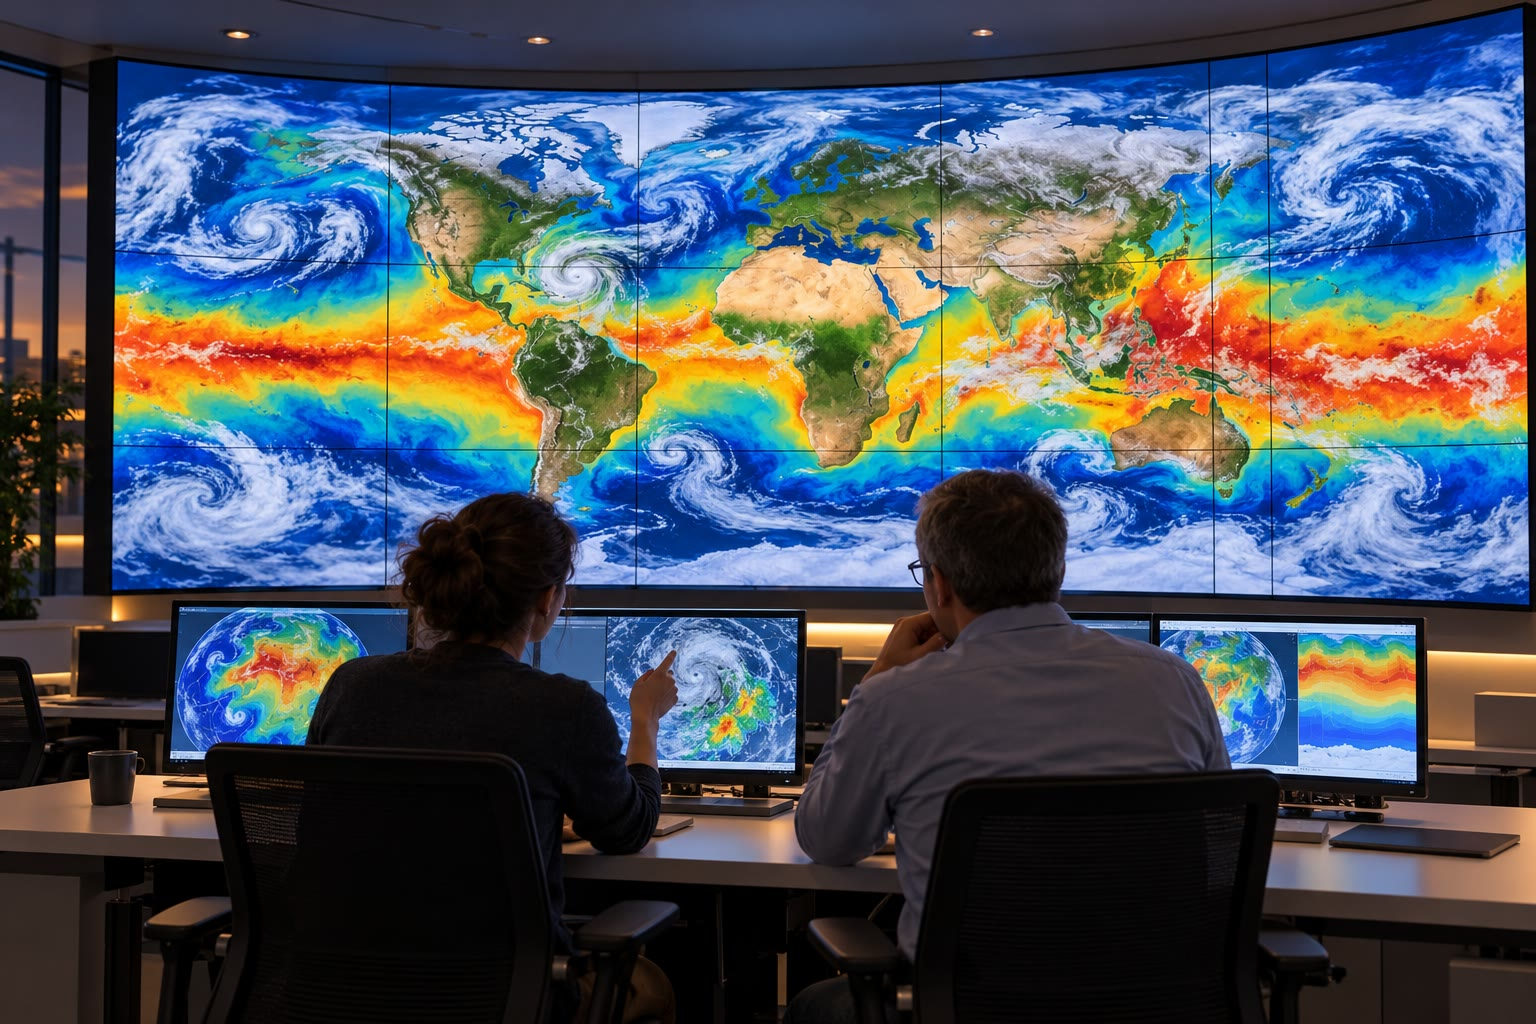
\includegraphics[width=\linewidth]{images/book5/ai/b3-model-centre.jpg}

{\scriptsize 两位科学家站在一面屏幕墙前，屏幕上显示
模式运行的全球场（AI 生成的示意图）。}
\end{minipage}
\end{inthelab}
% ledger: ar6ch1:esm, ar6ch1:models

\section{练习}

\begin{exercise}[$\star$]\label{exo:b3:climate-models:1}
布迪科 OLR 定律为 $I = a + bT - (a_1 + b_1T)n$，其中 $a = 14.0$，$b =
0.14$，$a_1 = 3.0$，$b_1 = 0.10$，OLR 以 \unit{kcal.cm^{-2}} 每月计，$T$
以 \unit{\celsius} 计。取云量 $n = 0.5$，求 $A$ 与 $B$，并
将其换算为 \unit{W/m^2} 与 \unit{W.m^{-2}.\celsius^{-1}}，
其中一个月取为一年的十二分之一，一年按 365.25 天计。该定律在
\qty{15}{\celsius} 时给出的 OLR 为多少？
\end{exercise}
% ledger: budyko69:olr

\begin{exercise}[$\star$]\label{exo:b3:climate-models:2}
已知 $Q = \qty{340}{W/m^2}$，$A = \qty{211.9}{W/m^2}$ 与 $B =
\qty{1.816}{W.m^{-2}.\celsius^{-1}}$，求反照率为 0.30 与 0.31 时的平衡温度。
反照率增加 0.01 时，该行星
会降温多少？
\end{exercise}

\begin{exercise}[$\star$]\label{exo:b3:climate-models:3}
求海水混合层单位面积的热容。该混合层厚
\qty{60}{m}，$\rho = \qty{1025}{kg/m^3}$ 与 $c_p = \qty{3992}{J.kg^{-1}.K^{-1}}$，
分别以 \unit{J.m^{-2}.K^{-1}} 与 \unit{W.\text{年}.m^{-2}.K^{-1}} 表示。
求\cref{thm:b3:climate-models:response}的响应时间，分别取 $\lambda = -B =
\qty{-1.816}{W.m^{-2}.\celsius^{-1}}$ 与 $\lambda =
\qty{-1.33}{W.m^{-2}.\celsius^{-1}}$。
\end{exercise}
% ledger: teos10:cp0

\begin{exercise}[$\star$]\label{exo:b3:climate-models:4}
对于 $\lambda = \qty{-1.33}{W.m^{-2}.\celsius^{-1}}$、
$\gamma = \qty{0.62}{W.m^{-2}.\celsius^{-1}}$ 与 $F_{2\times} =
\qty{3.93}{W/m^2}$ 的双层模式，求平衡气候敏感度 ECS、近似瞬态气候响应 TCR $F_{2\times}/
(\gamma - \lambda)$，以及二者之比。
\end{exercise}
% ledger: ar6sm7:two-layer, ipcc:erf-2xco2

\begin{exercise}[$\star\star$]\label{exo:b3:climate-models:5}
在正文的零维模式中，取太阳常数为
\qty{1340}{W/m^2}。求三个平衡态及各自净通量的斜率 $N'(T)$，
并判断哪些平衡态是稳定的。
\end{exercise}

\begin{exercise}[$\star\star$]\label{exo:b3:climate-models:6}
改动正文中的反照率斜坡：$\alpha = 0.62$，低于 \qty{-20}{\celsius} 时取值，
高于 \qty{0}{\celsius} 时取 $0.30$，两者之间线性变化。保持 $A$ 与 $B$ 不变，暖分支在何种太阳常数下终止，
该点比 \qty{1360}{W/m^2} 低百分之多少？
雪球地球在何种太阳常数下融化？
阈值的大小由什么决定？
\end{exercise}

\begin{exercise}[$\star\star$]\label{exo:b3:climate-models:7}
一个具有正文参数的模式行星处于雪球状态。
(a)~在今日太阳常数下，其温度为多少？(b)~保持太阳不变，
需要多大的强迫 $F$，才能使雪球的温度升至
\qty{-10}{\celsius}？该强迫是二氧化碳加倍强迫
\qty{3.93}{W/m^2} 的多少倍？(c)~冰层消失后，
若随即撤去强迫，行星将稳定在何处？
\end{exercise}
% ledger: ipcc:erf-2xco2, hoffman17:hysteresis

\begin{exercise}[$\star\star$]\label{exo:b3:climate-models:8}
模式 X 为一个虚构的双层模式，其中 $C = 7.0$，$C_d =
\qty{90}{W.\text{年}.m^{-2}.\celsius^{-1}}$，$\gamma = 0.70$ 与 $\lambda =
\qty{-1.10}{W.m^{-2}.\celsius^{-1}}$。精确计算其两个时间尺度，
并利用\cref{thm:b3:climate-models:two-layer}中的近似计算，
求份额 $a_f$、ECS 与近似 TCR。
\end{exercise}

\begin{exercise}[$\star\star$]\label{exo:b3:climate-models:9}
在正文的布迪科模式中，$\bar T = \qty{12.81}{\celsius}$，$\beta =
\qty{3.74}{W.m^{-2}.\celsius^{-1}}$，冰线位于 \ang{72}，在赤道处 $s = 1.221$，
极地处则为 $0.506$，$\alpha = 0.30$ 与 $0.62$。
求赤道与极地的温度，以及输送过程在两处
每平方米带走或带来的热量
$\beta(T - \bar T)$。
\end{exercise}

\begin{exercise}[$\star\star\star$]\label{exo:b3:climate-models:10}
一个无冰行星（处处 $\alpha = 0.30$）具有扩散输送
$D = -\mathcal D\,\partial_x[(1 - x^2)\partial_xT]$ 与日射分布
$s(x) = 1 + s_2P_2(x)$，其中 $P_2 = (3x^2 - 1)/2$。(a)~证明
$\partial_x[(1 - x^2)\partial_xP_2] = -6P_2$。(b)~证明 $T = T_0 +
T_2P_2(x)$ 为稳态解，其中 $T_0 = (Q(1 - \alpha) - A)/B$ 且
$T_2 = Qs_2(1 - \alpha)/(B + 6\mathcal D)$。(c)~再分析资料的
日射给出 $s_2 = \num{-0.476}$。若不计输送，
赤道与极地之间的温差为多少？(d)~$\mathcal D$ 取何值时
可得观测温差 \qty{55.3}{\celsius}？
\end{exercise}
% ledger: data:b3-ncep, data:b5-ncep-air

\begin{exercise}[$\star\star\star$]\label{exo:b3:climate-models:11}
(a)~将\cref{thm:b3:climate-models:two-layer}中的二次方程写成 $r^2 -
\Sigma r + \Pi = 0$，并证明：若 $4\Pi \ll \Sigma^2$，则其根
近似为 $\Sigma$ 与 $\Pi/\Sigma$。(b)~对随时间线性增长的强迫 $F = kt$，
证明当 $t \gg \tau_f$ 且 $T_d$ 仍较小时，
$T \approx kt/(\gamma - \lambda)$；由此推出近似的 TCR。(c)~检验
正文中的数值：$\Sigma$、$\Pi$、两个时间尺度，以及比值
$4\Pi/\Sigma^2$。
\end{exercise}
% ledger: ar6sm7:two-layer

\begin{exercise}[$\star\star\star$]\label{exo:b3:climate-models:12}
一组虚构的八个模式给出当前气候的可观测量 $X$ 及其
ECS：
\begin{center}
\begin{tabular}{l*{8}{c}}
\hline
$X$ & 0.2 & 0.5 & 0.6 & 0.8 & 1.0 & 1.1 & 1.3 & 1.5\\
ECS（\unit{\celsius}）& 2.3 & 2.7 & 3.1 & 3.2 & 3.8 & 3.9 & 4.4 & 4.6\\
\hline
\end{tabular}
\end{center}
(a)~求该集合中 ECS 的平均值与标准差。(b)~以最小二乘法拟合
ECS $= a + bX$，求相关系数与
残差的标准差。(c)~观测得 $X$ 为 $0.7
\pm 0.1$。该约束给出的 ECS 为多少，其分散范围如何？
(d)~什么情况会让你怀疑这一约束？
\end{exercise}
% ledger: ar6ch7:emergent

\section{问题：距离雪球有多近？}

\begin{problem}[{周末问题——平衡、稳定性与模型行星的
冰封阈值}]
\label{pb:b3:climate-models:1}
一颗模型行星的今日太阳常数为 $S_0 = \qty{1360}{W/m^2}$，
OLR 定律为 $A + BT$，其中 $A = \qty{211.9}{W/m^2}$，$B =
\qty{1.816}{W.m^{-2}.\celsius^{-1}}$。模型的反照率在
\qty{-10}{\celsius} 以下为 0.62，\qty{+10}{\celsius} 以上为 0.30，之间线性过渡，且
地表热容 $C = \qty{8.1}{W.\text{年}.m^{-2}.\celsius^{-1}}$。取
$\sigma = \qty{5.670e-8}{W.m^{-2}.K^{-4}}$。

\medskip\noindent\textbf{第一部分——处于平衡的行星。}
\begin{enumerate}
\item 求行星每平方米的平均日照量 $Q_0$，并
  说明其中的因子。
\item 求反照率为 0.30 时的吸收日照量，以及
  \qty{15}{\celsius} 时的 OLR。
\item 求暖平衡。
\item 求雪球平衡，并验证它位于
  冰态分支上。
\item 求位于反照率斜坡上的第三个平衡。
\item 求使吸收的日照以黑体形式
  返回太空的发射温度，并与暖平衡比较。
\end{enumerate}

\medskip\noindent\textbf{第二部分——稳定性与时间。}
\begin{enumerate}[resume]
\item 求各平衡处净通量的斜率 $N'(T)$，并
  说明哪些平衡是稳定的。
\item 偏离中间平衡的小扰动按 $\mathrm
  e^{t/\tau}$ 增长，求 $\tau$。
\item 求暖平衡的响应时间。
\item 施加一个 \qty{3.93}{W/m^2} 的强迫（二氧化碳加倍时的强迫），
  开启后求平衡时的升温，并与真实气候评估的
  ECS 进行比较。
\item 模式完成 \qty{95}{\percent} 的
  升温需要多长时间？真实气候为何需要更长时间？
\end{enumerate}

\medskip\noindent\textbf{第三部分——\omterm{def:b3:climate-models:multiple-equilibria}{鞍结分岔}。}
\begin{enumerate}[resume]
\item 随着太阳变暗，暖平衡在何温度与中间平衡
  相遇？求此处的 $Q$。
\item 求分岔点处的太阳常数，以及相对今日的
  下降百分比。
\item 刚低于该点时，气候会去向何处？求其温度。
\item 求雪球融化时的太阳常数，以及相对今日的
  上升百分比。
\item 画出 $S_0$ 先降至分岔点以下、再回升至
  \qty{1360}{W/m^2} 时温度所经历的回线示意图。
\end{enumerate}

\medskip\noindent\textbf{第四部分——冰线。}为该行星给出布迪科纬度模型，
取 $\beta = \qty{3.739}{W.m^{-2}.\celsius^{-1}}$，
冰反照率：冰线向极一侧为 0.62，向赤道一侧为 0.30，在
冰线边缘为 0.50，日射量取再分析资料的值：
\begin{center}
\begin{tabular}{lccccccc}
\hline
纬度 & \ang{0} & \ang{30} & \ang{40} & \ang{47.5} & \ang{55} & \ang{60} & \ang{72}\\
$s(x_s)$ & 1.2211 & 1.0730 & 0.9647 & 0.8688 & 0.7650 & 0.6947 & 0.5643\\
$F(x_s)$ & 0 & 0.5865 & 0.7324 & 0.8192 & 0.8863 & 0.9205 & 0.9738\\
\hline
\end{tabular}
\end{center}
\begin{enumerate}[resume]
\item 冰线位于 \ang{72} 时，求平均反照率 $\bar\alpha$
  和平均温度 $\bar T$。
\item 求今日使边缘位于 \ang{72} 的临界温度 $T_c$，
  并与再分析的 \qty{-15.8}{\celsius} 比较。
\item 在\cref{prop:b3:climate-models:iceline}中求 $Q(x_s)$ 的分子
  以及比值 $\beta/B$。
\item 求冰线位于 \ang{30}、\ang{40}、
  \ang{47.5}、\ang{55} 和 \ang{60} 时的 $Q(x_s)/Q_0$。
\item 这些值的最小值位于何处？哪些冰线是稳定的？
\item 在今日太阳条件下，模式还允许哪一条冰线？它是否
  稳定？今日是否可能出现雪球？（使用 \ang{0} 一列的数据。）
\item 将纬度模型的阈值与第~III~部分中的阈值
  及布迪科的 \qty{1.6}{\percent} 进行比较，并将阈值处冰的纬度
  与他给出的 \ang{50} 进行比较。
\item 给出使模型行星冰封的太阳常数下降量（以百分比计），
  保留两位有效数字。
\end{enumerate}
\end{problem}
% ledger: nasa:solar-mean, data:b5-ncep-air, data:b3-ncep, budyko69:transport, budyko69:albedo, budyko69:threshold, ipcc:ecs, const:sigma
